\documentclass[a4paper]{article}

\usepackage[utf8]{inputenc}
\usepackage[spanish]{babel}
\usepackage{graphics}
\usepackage{caption}
\usepackage{subcaption}
\usepackage[demo]{graphicx}
\usepackage{enumitem}
\usepackage{longtable}
\usepackage{listings}
\usepackage{listingsutf8}
\usepackage{framed}
\usepackage{float}
\usepackage{hyperref}
\usepackage{amsmath}

\begin{document}

\begin{titlepage}

\begin{center}
\vspace*{1.5in}
\vspace*{-1in}
\begin{figure}[htb]
\begin{center}

\includegraphics[width=8cm]{logoUZ.png}
\end{center}
\end{figure}

\vspace*{0.3in}

Universidad de Zaragoza \\

\vspace*{0.3in}

\begin{large}
VIDEOJUEGOS\\
\end{large}
\vspace*{0.2in}
\begin{Large}
\textbf{Super Bomberman} \\
\end{Large}
\vspace*{0.3in}
\begin{large}
\end{large}
\vspace*{0.1in}
\rule{80mm}{0.1mm}\\
\vspace*{0.1in}
\begin{large}
Hecho por: \\
Jaime Ruiz-Borau Vizárraga (546751) \\
Patricia Lázaro Tello (554309) \\

\end{large}
\end{center}

\end{titlepage}
\tableofcontents

\newpage
\section{Descripción del videojuego realizado}
\paragraph{}Como se describe en el título de la memoria, el videojuego clásico elegido para la elaboración de un clon es el \textbf{Bomberman}. Dada la elevada similitud de mecánica, enemigos y objetivos entre las distintas entregas de Bomberman, se optó por implementar la mecánica del \textbf{primer Bomberman} que salió al mercado. Sin embargo, los sprites y las imágenes empleadas para el juego son de entregas de Bomberman posteriores.
\vspace*{0.2in}
\begin{figure}[H]
	\centering
	\begin{minipage}[b]{0.4\textwidth}
		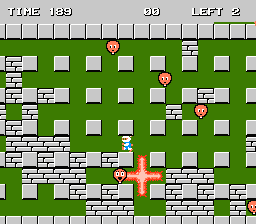
\includegraphics[width=\textwidth]{primerBomberman.png}
		\caption{Bomberman clásico}
	\end{minipage}
	\hfill
	\begin{minipage}[b]{0.4\textwidth}
		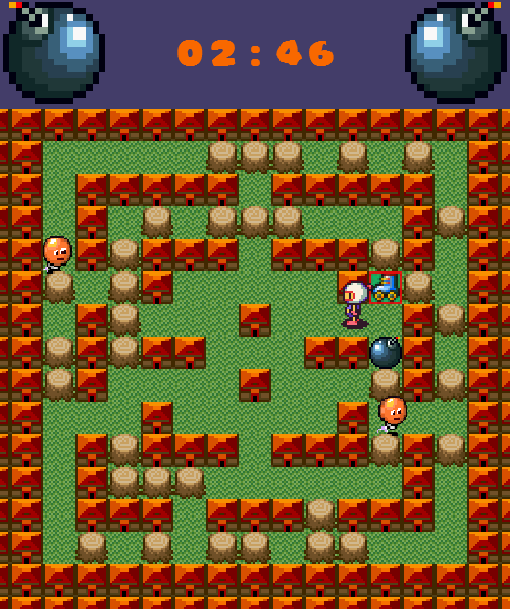
\includegraphics[width=\textwidth]{bomberman.png}
		\caption{Clon desarrollado}
	\end{minipage}
	\label{fig:primerBomberman}
\end{figure}
La única diferencia con el original es que la puntuación no se muestra hasta el final de la partida. También se ha implementado un menú con opciones para regular el volumen de la música del juego y la posibilidad de configurar los controles del juego.
\newpage
\section{Detalles de la implementación en 2D}
\paragraph{}Para el juego en 2D se implementó un motor gráfico basado en un hilo principal renderizando frames a razón de 60 por segundo, mostrando los distintos sprites del juego utilizando las funciones estándar de Java para mostrar gráficos por pantalla.
\paragraph{}El juego actualmente tiene 10 niveles generados aleatoriamente: posee unos mapas predefinidos de bloques no destruibles y dispone de forma aleatoria los enemigos y los bloques destruibles. Dichos bloques soltarán también de forma aleatoria los \textit{power-ups} mencionados anteriormente. Se obtienen puntos por destruir enemigos, por destruir bloques y por terminar niveles, y al terminar la partida, ya sea por acabar los 10 niveles o por morir a manos de un enemigo o una bomba, se muestra la tabla de mejores puntuaciones junto a la puntuación de dicha partida.
\begin{figure}[H]
	\centering
	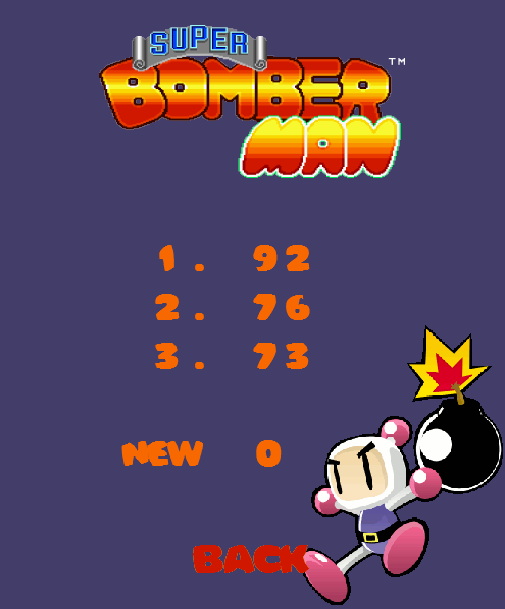
\includegraphics[width=2in]{score.png}
	\caption{Pantalla de puntuación}
	\label{fig:score}
\end{figure}
\paragraph{}Bomberman, el personaje que controla el jugador, puede moverse hacia arriba, abajo y hacia los lados; no puede atravesar bloques de ningún tipo y morirá si toca algún enemigo o la explosión de alguna bomba. Sin embargo, puede poner bombas para abrirse camino entre los bloques destruibles y eliminar los enemigos que salgan a su paso.
\paragraph{}La IA de los enemigos se ha implementado siguiendo las líneas del Bomberman clásico: patrones aleatorios de desplazamiento de los enemigos. Se ha optado por no implementar una IA más compleja ya que resultaba frustrante no poder acertarle a los enemigos y resultaba muy complicado el ganar las partidas, además de que el juego original no contaba con esa IA avanzada.
\paragraph{}Inicialmente las bombas tienen un radio de explosión de 1 casilla, sólo es posible poner una bomba a la vez en el escenario y Bomberman se mueve relativamente despacio. 
\newpage
\paragraph{}Sin embargo, conforme vaya obteniendo \textit{power ups}, el radio de las bombas cada vez es mayor, es posible poner más bombas en el escenario y Bomberman se irá moviendo más rápido, según el tipo de \textit{power up} que recoja.
\begin{figure}[H]
	\centering
	\begin{minipage}[b]{0.4\textwidth}
		\centering
		
\includegraphics[width=0.3\textwidth]{fuego.png}
		\caption{Power up que aumenta el radio de explosión de las bombas}
	\end{minipage}
	\hfill
	\begin{minipage}[b]{0.4\textwidth}
		\centering
		
\includegraphics[width=0.3\textwidth]{bomba.png}
		\caption{Power up que aumenta el número máximo de bombas en el escenario}
	\end{minipage}
	\hfill
	\begin{minipage}[b]{0.4\textwidth}
		\centering
		
\includegraphics[width=0.3\textwidth]{patines.png}
		\caption{Power up que aumenta la velocidad de Bomberman}
	\end{minipage}
	\label{fig:powerups}
\end{figure}
\paragraph{}El juego también contiene un menú principal desde el que se puede acceder a todos los apartados del mismo: 
\begin{itemize}
	\item Juego en 2D
	\item Juego en 3D
	\item Opciones de sonido
	\item Opciones de controles
	\item Ranking
	\item Créditos
\end{itemize}
\begin{figure}[H]
	\centering
	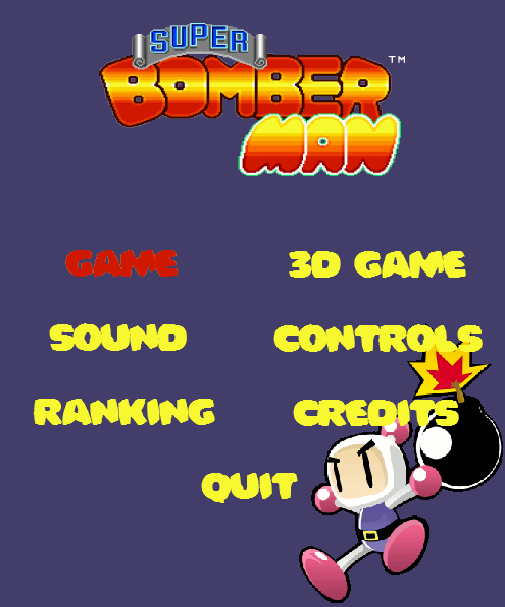
\includegraphics[width=2in]{menuses.png}
	\caption{Pantalla principal}
	\label{fig:menuses}
\end{figure}
\newpage
\section{Detalles de la implementación en 3D}
\paragraph{}En cuanto a la implementación del juego en 3D, se ha optado por utilizar una librería apta para el lenguaje Java; se trata de \textbf{libgdx}.
\paragraph{}Esta librería permite cargar modelos 3D en el juego, así como utilizar y mover una cámara por el mundo 3D. Se han utilizado modelos de cubos para los bloques, enemigos, power ups y para Bomberman, variando únicamente en el color para distinguirlos. Para las bombas y sus explosiones se han utilizado esferas y cilindros, respectivamente.
\begin{figure}[H]
	\centering
	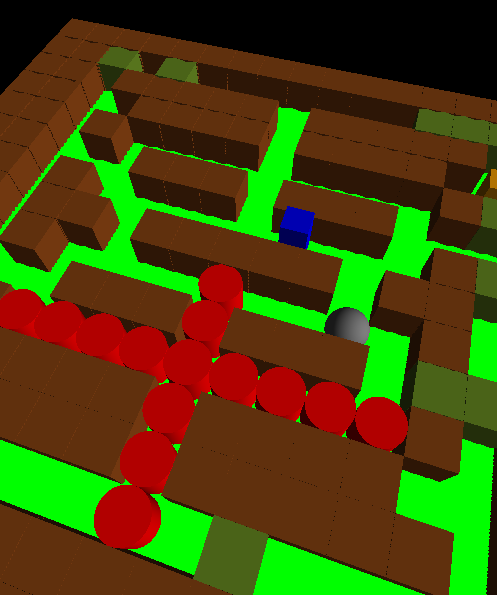
\includegraphics[width=2in]{bombermantresdes.png}
	\caption{Pantalla del juego en 3D}
	\label{fig:tresdes}
\end{figure}
Todo el sistema de juego 3D funciona exactamente igual que el 2D, únicamente cambia su aspecto visual. Sin embargo, solo se ha implementado un nivel en la versión 3D.
\newpage
\begin{thebibliography}{99}
	\bibitem{fig:primerBomberman} \textbf{Imágenes del primer Bomberman} - By Source, Fair use, [\url{https://en.wikipedia.org/w/index.php?curid=12465479}]
	\bibitem{} \textbf{Enlace al repositorio de Github} - [\url{https://github.com/EquipoJP/SuperBomberman}]
	\bibitem{} \textbf{Descargas del juego} - [\url{https://github.com/EquipoJP/SuperBomberman/releases}]
	

\end{thebibliography}

\end{document}